 \let\negmedspace\undefined
\let\negthickspace\undefined
\documentclass[journal]{IEEEtran}
\usepackage[a5paper, margin=10mm, onecolumn]{geometry}
%\usepackage{lmodern} % Ensure lmodern is loaded for pdflatex
\usepackage{tfrupee} % Include tfrupee package

\setlength{\headheight}{1cm} % Set the height of the header box
\setlength{\headsep}{0mm}     % Set the distance between the header box and the top of the text

\usepackage{gvv-book}
\usepackage{gvv}
\usepackage{cite}
\usepackage{amsmath,amssymb,amsfonts,amsthm}
\usepackage{algorithmic}
\usepackage{graphicx}
\usepackage{textcomp}
\usepackage{xcolor}
\usepackage{txfonts}
\usepackage{listings}
\usepackage{enumitem}
\usepackage{mathtools}
\usepackage{gensymb}
\usepackage{comment}
\usepackage[breaklinks=true]{hyperref}
\usepackage{tkz-euclide} 
\usepackage{listings}
% \usepackage{gvv}                                        
\def\inputGnumericTable{}                                 
\usepackage[latin1]{inputenc}                                
\usepackage{color}                                            
\usepackage{array}                                            
\usepackage{longtable}                                       
\usepackage{calc}                                             
\usepackage{multirow}                                         
\usepackage{hhline}                                           
\usepackage{ifthen}
\usepackage{lscape}
\begin{document}

\bibliographystyle{IEEEtran}



\title{1.10.20}
\author{EE25BTECH11057 - Rushil Shanmukha Srinivas
}
% \maketitle
% \newpage
% \bigskip
{\let\newpage\relax\maketitle}

\renewcommand{\thefigure}{\theenumi}
\renewcommand{\thetable}{\theenumi}
\setlength{\intextsep}{10pt} % Space between text and floats

\numberwithin{equation}{enumi}
\numberwithin{figure}{enumi}
\renewcommand{\thetable}{\theenumi}

\textbf{Question} : Find the direction cosines of the line passing through the two points (-2,4,-5) and (1,2,3).

\textbf{Solution} : 

\begin{table}[h!]
\centering
\begin{center}
    \begin{tabular}{|c|c|c|} 
        \hline
            \textbf{Variable} & \textbf{Parameter} & \textbf{Value} \\ 
        \hline
            $\lVert \vec{B - A}\rVert$ & c & 5 cm \\ 
        \hline
             $\lVert \vec{C - B}\rVert$ & a & - \\ 
        \hline
             $\lVert \vec{C - A}\rVert$ & b &   -    \\
        \hline
            $\angle \vec{A}$  & -  & $45^\circ$ \\
        \hline
    \end{tabular}
\end{center}  

\caption{Variables used}
\end{table}
Let
\begin{align}
\vec{A}=\myvec {-2 \\ 4 \\ -5} ,\quad
\vec{B}=\myvec {1 \\ 2 \\ 3} .
\end{align}


Thus the direction (difference) vector of the line is
\begin{align}
\vec{v}=\vec{B}-\vec{A} =\myvec {3 \\ -2 \\ 8} .
\end{align}

The length of $\vec{v}$ is
\begin{align*}
\vec{v}^\top \vec{v} &= \myvec{3 & -2 & 8}\myvec{3 \\ -2 \\ 8} \\
&= 3^3 + \brak{-2}^2 + \brak{8}^2 \\
&= 9 + 4 + 64 = 77
\end{align*}

Therefore, the norm of $\vec{v}$ is
\begin{align*}
\norm{\vec{v}} &\overset{\Delta}{=} \sqrt{\vec{v}^\top \vec{v}} = \sqrt{77} 
\end{align*} 

The unit vector in the direction of $\vec{v}$ is  

\begin{align*} 
\frac{\vec{v}}{\norm{\vec{v}}}
&= \frac{1}{\sqrt{77}}\myvec{3 \\ -2 \\ 8}
\end{align*}

Let $\alpha,\beta,\gamma$ be the angles made by the line with the $x,y,z$ axes respectively.Then, the direction cosines are the elements of the above direction vector
\begin{align*}
\cos\alpha = \frac{3}{\sqrt{77}}, \quad
\cos\beta = -\frac{2}{\sqrt{77}}, \quad
\cos\gamma = \frac{8}{\sqrt{77}}
\end{align*}

\begin{figure}[h!]
  \centering
  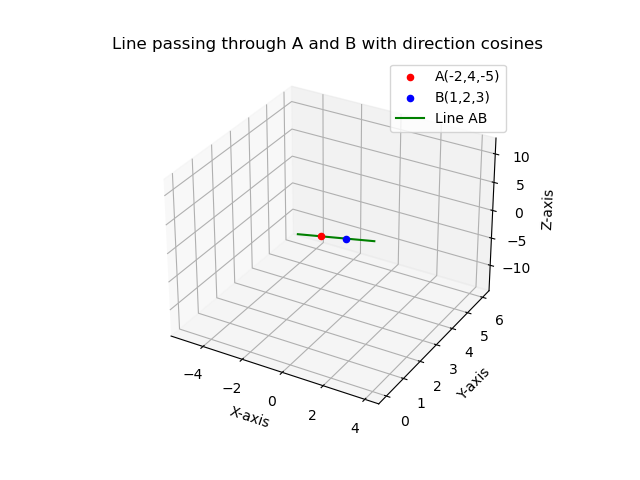
\includegraphics[width=0.9\columnwidth]{figs/fig_vector.png} 
   \caption*{Fig : Vector v}
  \label{Fig1}
\end{figure}


\end{document}








